\chapter{Resultados y discusión}
\label{ch:resultados}

En este capítulo se presentan los resultados obtenidos tras aplicar los distintos algoritmos de clasificación sobre los conjuntos de datos preparados en las fases anteriores. El objetivo principal es evaluar el rendimiento de cada modelo bajo diferentes escenarios y métricas, con el fin de identificar sus fortalezas y limitaciones en la detección de \textit{malware}.

\vspace{1em}

Para ello, se analizan tanto los experimentos realizados en el problema binario, donde se distingue entre \textit{software} malicioso y benigno, como en el problema multiclase, en el que se busca identificar el tipo específico de amenaza. Los clasificadores se evalúan considerando como métricas: la sensibilidad mínima, el Valor-F1 y la precisión de los modelos.

\vspace{1em}

Asimismo, se discute la capacidad de generalización de cada modelo, observando las diferencias de rendimiento entre los conjuntos de entrenamiento y prueba, así como la influencia de la variabilidad introducida por el desbalance de clases. Con este análisis se pretende ofrecer una visión comparativa que facilite la elección del modelo más adecuado en un contexto práctico de detección de amenazas.

\newpage
\section{Clasificación binaria}
\label{sec:clas_binaria}

En primer lugar se expondrán los resultados obtenidos en clasificación binaria.

\subsection{Árboles de decisión}
\label{subsec:dt_bin}

La tabla \ref{tabla:dt_bin} muestra los resultados de la clasificación binaria utilizando el modelo \textit{DecisionTreeClassifier}, evaluados en 10 ejecuciones distintas con diferentes estados.

\vspace{1em}

Para el entrenamiento, la precisión (\textit{Acc}), la sensibilidad mínima (\textit{MS}) y el \textit{Valor-F1} alcanzan valores muy próximos a 1 en todas las ejecuciones. En cuanto al test, la precisión oscila entre 0.942 y 0.953, mientras que la sensibilidad mínima se sitúa entre 0.935 y 0.946. El Valor-F1 se mantiene constante en 1 en todas las ejecuciones.

\vspace{1em}

El gráfico \ref{fig:dt_bin} compara la distribución de los valores de \textit{accuracy} en entrenamiento y en test para el clasificador basado en árboles de decisión. Se observa que en entrenamiento son consistentemente cercanos a 1, sin apenas variabilidad, lo que indica que el modelo es capaz de ajustarse casi perfectamente a los datos de entrenamiento.

\vspace{1em}

En contraste, los valores en test muestran una ligera caída, con una variabilidad mayor que en entrenamiento. Esta diferencia refleja que el modelo generaliza de forma aceptable, aunque la brecha respecto al rendimiento en entrenamiento sugiere la existencia de cierto sobreajuste.

\vspace{1em}

El uso combinado de violinplot y boxplot permite apreciar tanto la concentración de los valores en torno a la media como la dispersión entre diferentes ejecuciones. En este caso, el test mantiene una distribución compacta, sin valores atípicos extremos, lo que aporta robustez a la evaluación del modelo.

\begin{figure}[H]
	\centering
	% include first image
	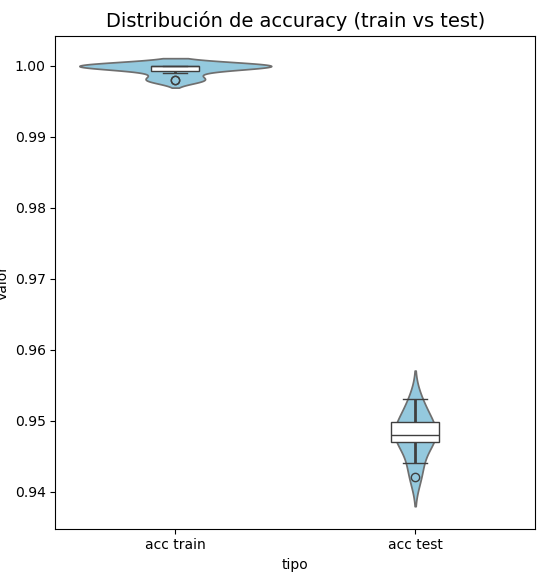
\includegraphics[width=1\linewidth]{Imagenes/dt_bin}
	\caption[Boxplot con violinplot para árboles de decisión]{Boxplot con violinplot para árboles de decisión}
	\label{fig:dt_bin}
\end{figure}

\begin{table}[H]
	\centering
	\begin{tabular}{ |c|c|c|c|c|c|c| }
		\hline
		\rowcolor{LightCyan}
		 & \multicolumn{3}{c|}{Entrenamiento} & \multicolumn{3}{c|}{Generalización} \\
		\hline
		\rowcolor{LightCyan}
		 Semilla & Acc & MS & F1 & Acc & MS & F1 \\
		\hline
		0    & \textbf{1.000} & \textbf{1.000} & \textbf{1.000} & \textit{0.951} & 0.942          & \textbf{1.000} \\
		1    & \textit{1.000} & \textit{1.000} & \textit{1.000} & 0.944          & 0.935          & \textit{1.000} \\
		2    & 1.000          & 1.000          & 1.000          & 0.942          & 0.935          & 1.000          \\
		3    & 1.000          & 1.000          & 1.000          & 0.948          & 0.938          & 1.000          \\
		4    & 1.000          & 1.000          & 1.000          & \textbf{0.953} & \textbf{0.946} & 1.000          \\
		5    & 0.998          & 0.997          & 1.000          & 0.947          & 0.936          & 1.000          \\
		6    & 0.998          & 0.997          & 1.000          & 0.947          & 0.941          & 1.000          \\
		7    & 1.000          & 1.000          & 1.000          & 0.949          & \textit{0.946} & 1.000          \\
		8    & 0.999          & 0.998          & 1.000          & 0.948          & 0.937          & 1.000          \\
		9    & 1.000          & 1.000          & 1.000          & 0.950          & 0.940          & 1.000          \\
		Mean & 0.999          & 0.999          & 1.000          & 0.948          & 0.940          & 1.000          \\
		STD  & 0.001          & 0.001          & 0.000          & 0.003          & 0.004          & 0.000          \\
		\hline
	\end{tabular}
	\caption{Clasificación binaria con \textit{DecisionTreeClassifier}}
	\label{tabla:dt_bin}
\end{table}

\subsection{\textit{Random forest}}
\label{subsec:rf_bin}

En la tabla \ref{tabla:rf_bin} se muestran los resultados de la clasificación binaria utilizando el modelo RandomForestClassifier para diferentes estados aleatorios.

\vspace{1em}

En el conjunto de entrenamiento, las métricas presentan valores altos y consistentes: la exactitud oscila entre 0.978 y 0.989, la métrica de sensibilidad mínima entre 0.920 y 0.956, y la puntuación F1 entre 0.988 y 0.992.

\vspace{1em}

En el conjunto de prueba, la exactitud mantiene valores muy estables alrededor de 0.936–0.941. La sensibilidad mínima muestra una mayor variabilidad, con valores que van desde 0.400 hasta 0.609, mientras que la métrica F1 se mantiene muy uniforme, entre 0.971 y 0.974.

\begin{figure}[H]
	\centering
	% include first image
	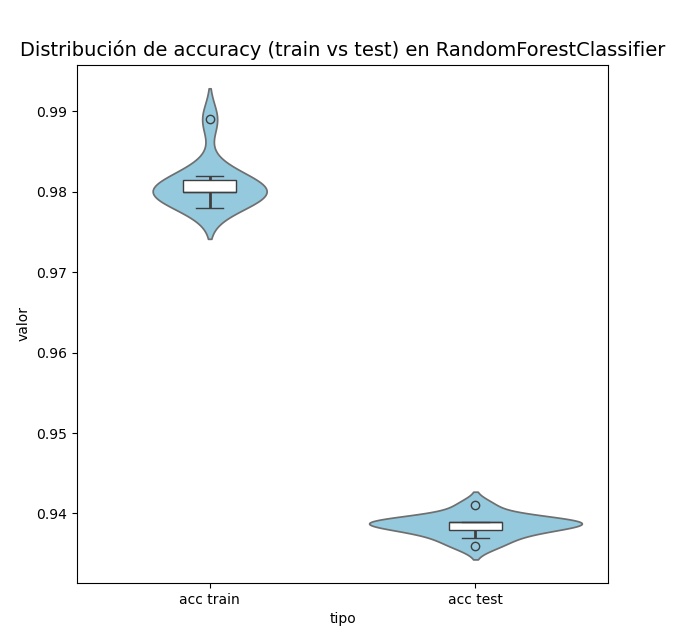
\includegraphics[width=1\linewidth]{Imagenes/rf_bin}
	\caption[Boxplot con violinplot para \textit{Random forest}]{Boxplot con violinplot para \textit{Random forest}}
	\label{fig:rf_bin}
\end{figure}

El modelo muestra un rendimiento muy alto y consistente en precisión tanto en el entrenamiento como en el test. En el gráfico \ref{fig:rf_bin}, se observa que la distribución de accuracy es estrecha, con valores muy concentrados en torno a 0.98 en entrenamiento y 0.94 en test, lo que indica estabilidad en ambas fases.

\vspace{1em}

El F1-Score también refleja una gran solidez, con valores prácticamente constantes en todas las ejecuciones, lo que sugiere un buen equilibrio entre precisión y exhaustividad en la clasificación de las dos clases.

\vspace{1em}

Sin embargo, la métrica de sensibilidad mínima (MS) introduce un matiz importante: aunque en entrenamiento se mantiene elevada con poca dispersión, en test presenta una gran variabilidad. El rango de valores oscila entre 0.400 y 0.609 según la semilla utilizada, lo que se traduce en distribuciones más amplias en los gráficos. Esto indica que, en algunos casos, el modelo no logra identificar de forma adecuada los ejemplos más difíciles de una de las clases, comprometiendo la robustez de la clasificación en escenarios concretos.

\begin{table}[H]
	\centering
	\begin{tabular}{ |c|c|c|c|c|c|c| }
		\hline
		\rowcolor{LightCyan}
		 & \multicolumn{3}{c|}{Entrenamiento} & \multicolumn{3}{c|}{Generalización} \\
		\hline
		\rowcolor{LightCyan}
		 Semilla & Acc & MS & F1 & Acc & MS & F1 \\
		\hline
		0    & 0.980          & 0.928          & 0.989          & 0.939          & 0.524          & 0.972          \\
		1    & 0.980          & 0.929          & 0.990          & \textit{0.939} & 0.500          & 0.973          \\
		2    & 0.980          & 0.927          & 0.989          & \textbf{0.941} & 0.429          & \textbf{0.974} \\
		3    & 0.979          & 0.923          & 0.989          & 0.939          & 0.444          & 0.973          \\
		4    & 0.982          & 0.931          & 0.990          & 0.939          & 0.500          & \textit{0.974} \\
		5    & 0.980          & 0.929          & 0.990          & 0.937          & \textbf{0.609} & 0.971          \\
		6    & 0.978          & 0.920          & 0.988          & 0.938          & 0.550          & 0.971          \\
		7    & 0.980          & 0.929          & 0.990          & 0.939          & \textit{0.562} & 0.972          \\
		8    & \textit{0.982} & \textit{0.934} & \textit{0.991} & 0.938          & 0.489          & 0.971          \\
		9    & \textbf{0.989} & \textbf{0.956} & \textbf{0.992} & 0.936          & 0.400          & 0.972          \\
		Mean & 0.981          & 0.931          & 0.990          & 0.939          & 0.501          & 0.972          \\
		STD  & 0.003          & 0.010          & 0.001          & 0.001          & 0.064          & 0.001          \\
		\hline
	\end{tabular}
	\caption{Clasificación binaria con \textit{RandomForestClassifier}}
	\label{tabla:rf_bin}
\end{table}

\newpage
\subsection{\textit{K-NN}}
\label{subsec:knn_bin}

En la tabla \ref{tabla:knn_bin} se muestran los resultados obtenidos con el clasificador KNeighborsClassifier bajo diferentes semillas.

\vspace{1em}

En la fase de entrenamiento, todas las semillas reportan valores de $\text{Acc}$, $\text{MS}$ y $\text{F1}$ iguales a 1.000, lo que refleja una completa uniformidad en las métricas. La media confirma este comportamiento perfecto, con desviaciones estándar nulas en las tres métricas.

\vspace{1em}

En la fase de generalización, la precisión presenta valores que oscilan entre 0.939 y 0.949, con una media de 0.947 y una desviación estándar reducida de 0.003. $\text{MS}$ toma valores entre 0.926 y 0.940, con una media de 0.934 y una desviación estándar de 0.004, mostrando ligeras variaciones según la semilla utilizada. Finalmente, $\text{F1}$ alcanza en todos los casos el valor de 1.000, con media y desviación estándar constantes.

\begin{table}[H]
	\centering
	\begin{tabular}{ |c|c|c|c|c|c|c| }
		\hline
		\rowcolor{LightCyan}
		 & \multicolumn{3}{c|}{Entrenamiento} & \multicolumn{3}{c|}{Generalización} \\
		\hline
		\rowcolor{LightCyan}
		 Semilla & Acc & MS & F1 & Acc & MS & F1 \\
		\hline
		0    & 1.000          & 1.000          & 1.000          & 0.947          & 0.935          & 1.000          \\
		1    & 1.000          & 1.000          & 1.000          & 0.949          & 0.938          & 1.000          \\
		2    & 1.000          & 1.000          & 1.000          & 0.939          & 0.926          & 1.000          \\
		3    & 1.000          & 1.000          & 1.000          & 0.949          & 0.937          & 1.000          \\
		4    & 1.000          & 1.000          & 1.000          & 0.949          & 0.936          & 1.000          \\
		5    & 1.000          & 1.000          & 1.000          & 0.946          & 0.932          & 1.000          \\
		6    & 1.000          & 1.000          & 1.000          & 0.946          & 0.931          & 1.000          \\
		7    & 1.000          & 1.000          & 1.000          & 0.944          & 0.934          & 1.000          \\
		8    & 1.000          & 1.000          & 1.000          & 0.947          & 0.935          & 1.000          \\
		9    & 1.000          & 1.000          & 1.000          & 0.949          & 0.940          & 1.000          \\
		Mean & 1.000          & 1.000          & 1.000          & 0.947          & 0.934          & 1.000          \\
		STD  & 0.000          & 0.000          & 0.000          & 0.003          & 0.004          & 0.000          \\
		\hline
	\end{tabular}
	\caption{Clasificación binara con \textit{KNeighborsClassifier}}
	\label{tabla:knn_bin}
\end{table}

\newpage
El gráfico \ref{fig:knn_bin} muestra como para el entrenamiento, todos los valores de \textit{accuracy} se encuentran exactamente en 1.000, lo que se refleja en el \texttt{violinplot} como una única línea y en el \texttt{boxplot} como una caja colapsada. Esto indica que el modelo clasifica perfectamente todos los patrones del conjunto de entrenamiento en cada ejecución.

\vspace{1em}

Para la generalización, los valores oscilan ligeramente entre 0.939 y 0.949. El \texttt{violinplot} muestra una distribución muy estrecha alrededor de la media, y el \texttt{boxplot} confirma que la mediana es cercana a 0.947, con una ligera variabilidad reflejada por los bigotes.

\vspace{1em}

Se aprecia un entrenamiento perfecto y una generalización muy alta y consistente, con poca dispersión en los resultados de test, aunque podemos ver una ligera caída en las métricas.

\begin{figure}[H]
	\centering
	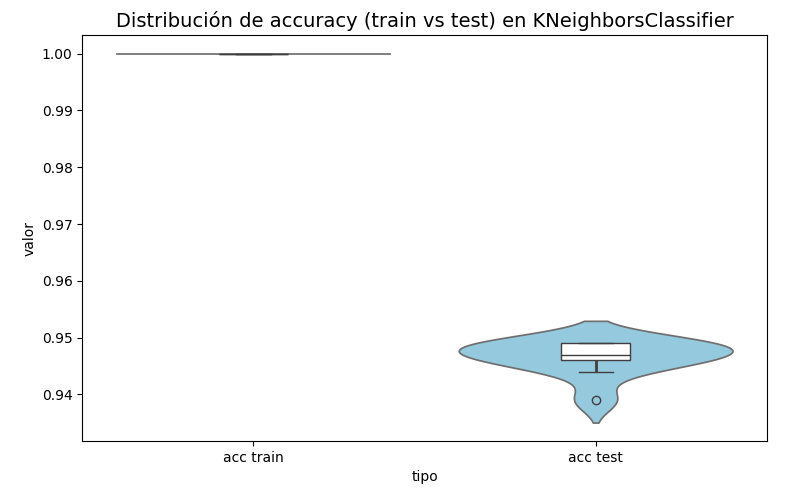
\includegraphics[width=1\linewidth]{Imagenes/knn_bin}
	\caption[Boxplot con violinplot para \textit{K-NN}]{Boxplot con violinplot para \textit{K-NN}}
	\label{fig:knn_bin}
\end{figure}

Para ver más clara la caída en las métricas anteriores, podemos hacer uso de las matrices de confusión reflejadas en la figura \ref{figT:knn_mat}. En ella podemos ver que la clasificación en entrenamiento es perfecta, acertando en todos los patrones, mientras que el para la generalización los resultados son peores por un aumento significativo de los falsos positivos y los falsos negativos. Esto podría significar un ligero sobreajuste del modelo.

\begin{figure}[H]
	\begin{subfigure}{.5\textwidth}
		\centering
		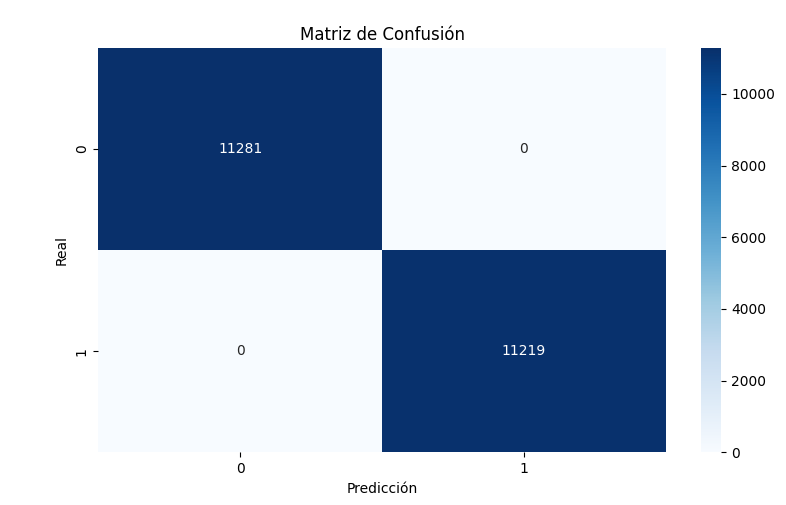
\includegraphics[width=1\linewidth]{Imagenes/knn_bin_mat_train}
		\caption{Título subfigura 1}
		\label{fig:sub-first}
	\end{subfigure}
	\begin{subfigure}{.5\textwidth}
		\centering
		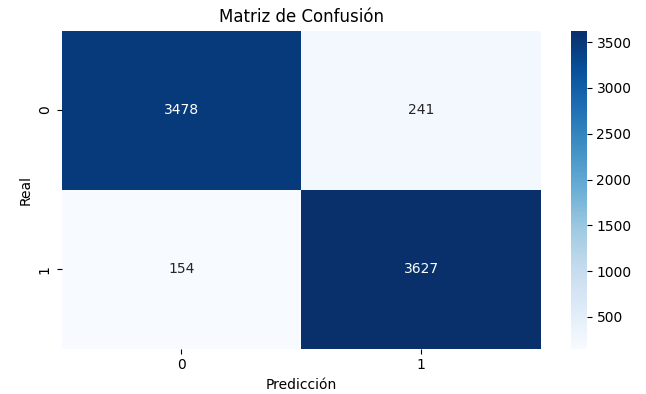
\includegraphics[width=1\linewidth]{Imagenes/knn_bin_mat_test}
		\caption{Título subfigura 2}
		\label{fig:sub-second}
	\end{subfigure}
	\caption[Matriz de confusión en \textit{K-NN}]{Matriz de confusión en \textit{K-NN}}
	\label{figT:knn_mat}
\end{figure}

\subsection{Máquinas de vectores de soporte}
\label{subsec:svm_bin}

En la tabla \ref{fig:svm_bin} podemos ver como para el conjunto de entrenamiento, la precisión se mantiene en valores cercanos a 0.76 en todas las ejecuciones, mientras que la mínima sensibilidad (MS) muestra variaciones entre 0.656 y 0.704.

\vspace{1em}

En el conjunto de generalización, todas las métricas presentan unos resultados muy similares a los de entrenamiento. Esto se puede apreciar claramente observando la desviación estándar (\textit{STD}), que indica una baja variabilidad en todas las métricas.

\begin{table}[H]
	\centering
	\begin{tabular}{ |c|c|c|c|c|c|c| }
		\hline
		\rowcolor{LightCyan}
		 & \multicolumn{3}{c|}{Entrenamiento} & \multicolumn{3}{c|}{Generalización} \\
		\hline
		\rowcolor{LightCyan}
		 Semilla & Acc & MS & F1 & Acc & MS & F1 \\
		\hline
		0 & 0.757 & 0.656 & 1.000 & 0.764 & 0.672 & 1.000 \\
		1 & 0.761 & 0.671 & 1.000 & 0.769 & 0.681 & 1.000 \\
		2 & 0.766 & 0.702 & 1.000 & 0.757 & 0.699 & 1.000 \\
		3 & 0.762 & 0.700 & 1.000 & 0.766 & 0.704 & 1.000 \\
		4 & 0.760 & 0.684 & 1.000 & 0.768 & 0.696 & 1.000 \\
		5 & 0.761 & 0.663 & 1.000 & 0.753 & 0.655 & 1.000 \\
		6 & 0.762 & 0.702 & 1.000 & 0.762 & 0.683 & 1.000 \\
		7 & 0.763 & 0.699 & 1.000 & 0.759 & 0.697 & 1.000 \\
		8 & 0.766 & 0.704 & 1.000 & 0.758 & 0.693 & 1.000 \\
		9 & 0.760 & 0.662 & 1.000 & 0.758 & 0.666 & 1.000 \\
		Mean & 0.762 & 0.684 & 1.000 & 0.762 & 0.685 & 1.000 \\
		STD & 0.003 & 0.020 & 0.000 & 0.005 & 0.016 & 0.000 \\
		\hline
	\end{tabular}
	\caption{Clasificación binaria con \textit{SVC}}
	\label{tabla:svm_bin}
\end{table}

Se muestran valores muy consistentes tanto en el conjunto de entrenamiento como en el de test. En el gráfico \ref{fig:svm_bin}, las distribuciones para ambos conjuntos aparecen concentradas en torno al 0.76, sin grandes variaciones entre diferentes semillas. Esto queda reforzado por la baja dispersión que se observa en el \texttt{boxplot} y por la forma compacta del \texttt{violinplot}, que refleja que no existen valores extremos significativos.

\vspace{1em}

Aunque no se han obtenido los mejores resultados con las máquinas de vectores de soporte, es interesante la estabilidad que consiguen a la hora de generalizar. Esta cercanía entre ambas distribuciones indica que el modelo mantiene un rendimiento estable al generalizar sobre datos no vistos.

\begin{figure}[H]
	\centering
	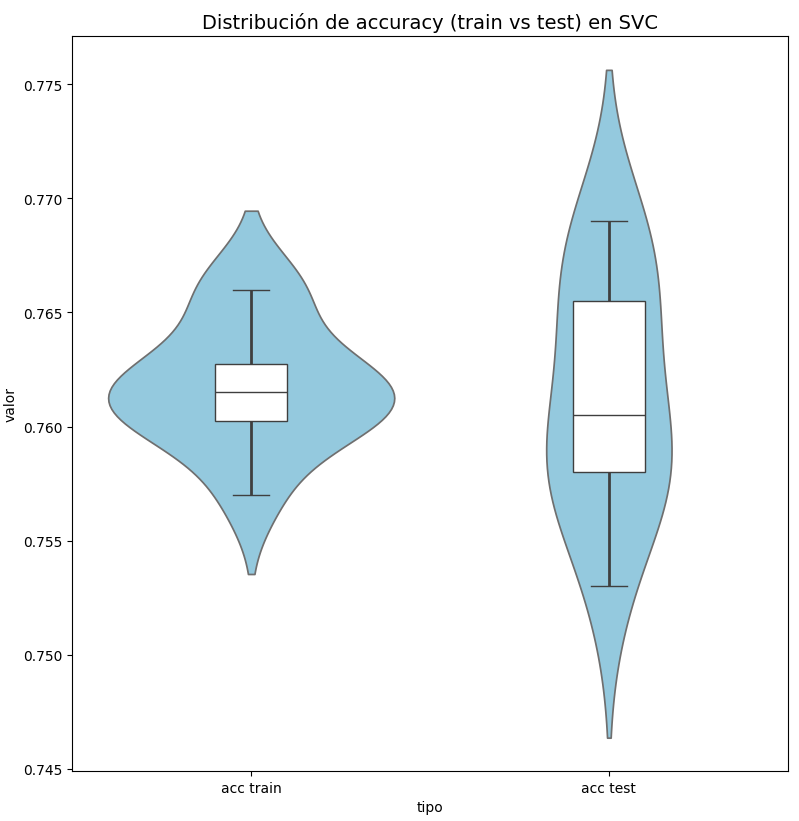
\includegraphics[width=1\linewidth]{Imagenes/svm_bin}
	\caption[Boxplot con violinplot para \textit{SVC}]{Boxplot con violinplot para \textit{SVC}}
	\label{fig:svm_bin}
\end{figure}

\newpage
\subsection{\textit{Ridge}}
\label{subsec:ridge_bin}

En los resultados obtenidos con el clasificador \textit{RidgeClassifier}, las métricas de entrenamiento muestran valores estables. La precisión se mantiene en un rango estrecho entre 0.645 y 0.652, con una media de 0.649 y una desviación estándar de 0.002. La mínima sensibilidad presenta mayor variabilidad, con valores comprendidos entre 0.549 y 0.573, alcanzando una media de 0.564 y una desviación estándar de 0.008.

\vspace{1em}

En el conjunto de generalización, la precisión presenta una media de 0.648, muy próxima a la de entrenamiento, y oscila entre 0.639 y 0.655, con una desviación estándar de 0.005. La mínima sensibilidad alcanza una media de 0.561, con valores entre 0.530 y 0.573 y una desviación estándar de 0.014.

\begin{table}[H]
	\centering
	\begin{tabular}{ |c|c|c|c|c|c|c| }
		\hline
		\rowcolor{LightCyan}
		 & \multicolumn{3}{c|}{Entrenamiento} & \multicolumn{3}{c|}{Generalización} \\
		\hline
		\rowcolor{LightCyan}
		 Semilla & Acc & MS & F1 & Acc & MS & F1 \\
		\hline
		0 & 0.649 & 0.549 & 1.000 & 0.648 & 0.530 & 1.000 \\
		1 & 0.645 & 0.558 & 1.000 & 0.655 & 0.569 & 1.000 \\
		2 & 0.652 & 0.573 & 1.000 & 0.645 & 0.564 & 1.000 \\
		3 & 0.649 & 0.567 & 1.000 & 0.653 & 0.570 & 1.000 \\
		4 & 0.651 & 0.573 & 1.000 & 0.651 & 0.573 & 1.000 \\
		5 & 0.647 & 0.562 & 1.000 & 0.648 & 0.558 & 1.000 \\
		6 & 0.648 & 0.556 & 1.000 & 0.650 & 0.573 & 1.000 \\
		7 & 0.651 & 0.571 & 1.000 & 0.650 & 0.573 & 1.000 \\
		8 & 0.651 & 0.564 & 1.000 & 0.639 & 0.551 & 1.000 \\
		9 & 0.650 & 0.563 & 1.000 & 0.645 & 0.551 & 1.000 \\
		Mean & 0.649 & 0.564 & 1.000 & 0.648 & 0.561 & 1.000 \\
		STD & 0.002 & 0.008 & 0.000 & 0.005 & 0.014 & 0.000 \\
		\hline
	\end{tabular}
	\caption{Clasificación binaria con \textit{RidgeClassifier}}
	\label{tabla:ridge_bin}
\end{table}

En el gráfico \ref{fig:ridge_bin}, se observa que ambos conjuntos presentan valores muy próximos. Las cajas muestran una dispersión reducida, con rangos estrechos tanto en entrenamiento como en test. Esto se traduce en que el modelo ofrece resultados consistentes sin grandes fluctuaciones entre diferentes semillas.

\vspace{1em}

La forma del \texttt{violinplot} refleja estabilidad en el rendimiento, con pequeñas variaciones entre ejecuciones.

\begin{figure}[H]
	\centering
	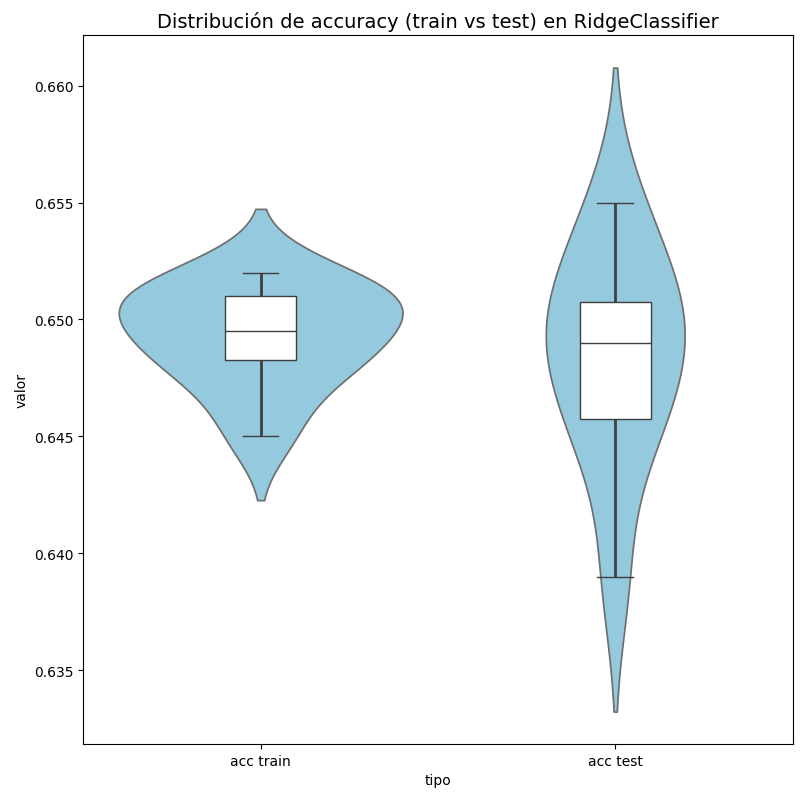
\includegraphics[width=1\linewidth]{Imagenes/ridge_bin}
	\caption[Boxplot con violinplot para \textit{RidgeClassifier}]{Boxplot con violinplot para \textit{RidgeClassifier}}
	\label{fig:ridge_bin}
\end{figure}

\subsection{Perceptrón multicapa}
\label{subsec:mlp_bin}

\begin{table}[H]
	\centering
	\begin{tabular}{ |c|c|c|c|c|c|c| }
		\hline
		\rowcolor{LightCyan}
		 & \multicolumn{3}{c|}{Entrenamiento} & \multicolumn{3}{c|}{Generalización} \\
		\hline
		\rowcolor{LightCyan}
		 Semilla & Acc & MS & F1 & Acc & MS & F1 \\
		\hline
		0 & 0.783 & 0.771 & 1.000 & 0.789 & 0.778 & 1.000 \\
		1 & 0.788 & 0.736 & 1.000 & 0.792 & 0.740 & 1.000 \\
		2 & 0.788 & 0.750 & 1.000 & 0.782 & 0.739 & 1.000 \\
		3 & 0.733 & 0.605 & 1.000 & 0.737 & 0.609 & 1.000 \\
		4 & 0.767 & 0.759 & 1.000 & 0.769 & 0.760 & 1.000 \\
		5 & 0.790 & 0.736 & 1.000 & 0.783 & 0.730 & 1.000 \\
		6 & 0.777 & 0.772 & 1.000 & 0.783 & 0.781 & 1.000 \\
		7 & 0.774 & 0.767 & 1.000 & 0.770 & 0.763 & 1.000 \\
		8 & 0.778 & 0.704 & 1.000 & 0.772 & 0.705 & 1.000 \\
		9 & 0.788 & 0.762 & 1.000 & 0.784 & 0.751 & 1.000 \\
		Mean & 0.776 & 0.736 & 1.000 & 0.776 & 0.736 & 1.000 \\
		STD & 0.017 & 0.051 & 0.000 & 0.016 & 0.050 & 0.000 \\
		\hline
	\end{tabular}
	\caption{Clasificación binaria con \textit{MLPClassifier}}
	\label{tabla:mlp_bin}
\end{table}


\subsection{\textit{Light gradient boosting machine}}
\label{subsec:lgbm_bin}

\begin{table}[H]
	\centering
	\begin{tabular}{ |c|c|c|c|c|c|c| }
		\hline
		\rowcolor{LightCyan}
		 & \multicolumn{3}{c|}{Entrenamiento} & \multicolumn{3}{c|}{Generalización} \\
		\hline
		\rowcolor{LightCyan}
		 Semilla & Acc & MS & F1 & Acc & MS & F1 \\
		\hline
		0 & 0.984 & 0.981 & 1.000 & 0.953 & 0.952 & 1.000 \\
		1 & 0.984 & 0.980 & 1.000 & 0.951 & 0.947 & 1.000 \\
		2 & 0.985 & 0.983 & 1.000 & 0.949 & 0.946 & 1.000 \\
		3 & 0.985 & 0.982 & 1.000 & 0.952 & 0.951 & 1.000 \\
		4 & 0.984 & 0.981 & 1.000 & 0.950 & 0.945 & 1.000 \\
		5 & 0.985 & 0.981 & 1.000 & 0.949 & 0.948 & 1.000 \\
		6 & 0.985 & 0.982 & 1.000 & 0.952 & 0.949 & 1.000 \\
		7 & 0.986 & 0.984 & 1.000 & 0.948 & 0.947 & 1.000 \\
		8 & 0.984 & 0.979 & 1.000 & 0.953 & 0.952 & 1.000 \\
		9 & 0.989 & 0.989 & 1.000 & 0.953 & 0.950 & 1.000 \\
		Mean & 0.985 & 0.982 & 1.000 & 0.951 & 0.949 & 1.000 \\
		STD & 0.002 & 0.003 & 0.000 & 0.002 & 0.002 & 0.000 \\
		\hline
	\end{tabular}
	\caption{Clasificación binaria con \textit{LGBMClassifier}}
	\label{tabla:lgbm_bin}
\end{table}

\subsection{Discusión de los resultados}
\label{subsec:discusion}

\section{Clasificación multiclase}
\label{sec:clas_multi}

\subsection{Árboles de decisión}
\label{subsec:dt_multi}

\begin{table}[th]
	\centering
	\begin{tabular}{ |c|c|c|c|c|c|c| }
		\hline
		\rowcolor{LightCyan}
		 & \multicolumn{3}{c|}{Entrenamiento} & \multicolumn{3}{c|}{Test} \\
		\hline
		\rowcolor{LightCyan}
		 Estado aleatorio & Acc & MS & F1 & Acc & MS & F1 \\
		\hline
		0 & 0.980 & 0.928 & 0.989 & 0.939 & 0.524 & 0.972 \\
		1 & 0.980 & 0.929 & 0.990 & 0.939 & 0.500 & 0.973 \\
		2 & 0.980 & 0.927 & 0.989 & 0.941 & 0.429 & 0.974 \\
		3 & 0.979 & 0.923 & 0.989 & 0.939 & 0.444 & 0.973 \\
		4 & 0.982 & 0.931 & 0.990 & 0.939 & 0.500 & 0.974 \\
		5 & 0.980 & 0.929 & 0.990 & 0.937 & 0.609 & 0.971 \\
		6 & 0.978 & 0.920 & 0.988 & 0.938 & 0.550 & 0.971 \\
		7 & 0.980 & 0.929 & 0.990 & 0.939 & 0.562 & 0.972 \\
		8 & 0.982 & 0.934 & 0.991 & 0.938 & 0.489 & 0.971 \\
		9 & 0.989 & 0.956 & 0.992 & 0.936 & 0.400 & 0.972 \\
		Mean & 0.981 & 0.931 & 0.990 & 0.939 & 0.501 & 0.972 \\
		STD & 0.003 & 0.010 & 0.001 & 0.001 & 0.064 & 0.001 \\
		\hline
	\end{tabular}
	\caption{Clasificación multiclase con \textit{DecisionTreeClassifier}}
	\label{tabla:dt_multi}
\end{table}


\subsection{\textit{Random forest}}
\label{subsec:rf_multi}

\begin{table}[th]
	\centering
	\begin{tabular}{ |c|c|c|c|c|c|c| }
		\hline
		\rowcolor{LightCyan}
		 & \multicolumn{3}{c|}{Entrenamiento} & \multicolumn{3}{c|}{Test} \\
		\hline
		\rowcolor{LightCyan}
		 Estado aleatorio & Acc & MS & F1 & Acc & MS & F1 \\
		\hline
		0 & 0.981 & 0.926 & 0.990 & 0.951 & 0.524 & 0.977 \\
		1 & 0.981 & 0.926 & 0.990 & 0.953 & 0.735 & 0.978 \\
		2 & 0.981 & 0.926 & 0.990 & 0.954 & 0.429 & 0.978 \\
		3 & 0.980 & 0.923 & 0.990 & 0.954 & 0.500 & 0.978 \\
		4 & 0.981 & 0.926 & 0.990 & 0.954 & 0.500 & 0.979 \\
		5 & 0.981 & 0.927 & 0.990 & 0.952 & 0.638 & 0.977 \\
		6 & 0.980 & 0.923 & 0.990 & 0.952 & 0.550 & 0.977 \\
		7 & 0.981 & 0.927 & 0.991 & 0.954 & 0.500 & 0.978 \\
		8 & 0.981 & 0.926 & 0.990 & 0.953 & 0.471 & 0.978 \\
		9 & 0.981 & 0.926 & 0.990 & 0.953 & 0.400 & 0.978 \\
		Mean & 0.981 & 0.926 & 0.990 & 0.953 & 0.525 & 0.978 \\
		STD & 0.000 & 0.002 & 0.000 & 0.001 & 0.098 & 0.001 \\
		\hline
	\end{tabular}
	\caption{Clasificación multiclase con \textit{RandomForestClassifier}}
	\label{tabla:rf_multi}
\end{table}


\subsection{\textit{K-NN}}
\label{subsec:knn_multi}

\begin{table}[th]
	\centering
	\begin{tabular}{ |c|c|c|c|c|c|c| }
		\hline
		\rowcolor{LightCyan}
		 & \multicolumn{3}{c|}{Entrenamiento} & \multicolumn{3}{c|}{Test} \\
		\hline
		\rowcolor{LightCyan}
		 Estado aleatorio & Acc & MS & F1 & Acc & MS & F1 \\
		\hline
		0 & 0.994 & 0.811 & 0.997 & 0.940 & 0.524 & 0.976 \\
		1 & 0.994 & 0.794 & 0.996 & 0.943 & 0.500 & 0.977 \\
		2 & 0.994 & 0.811 & 0.997 & 0.940 & 0.357 & 0.977 \\
		3 & 0.994 & 0.815 & 0.996 & 0.942 & 0.389 & 0.978 \\
		4 & 0.994 & 0.810 & 0.997 & 0.941 & 0.375 & 0.976 \\
		5 & 0.994 & 0.807 & 0.996 & 0.940 & 0.435 & 0.976 \\
		6 & 0.994 & 0.802 & 0.996 & 0.941 & 0.500 & 0.976 \\
		7 & 0.994 & 0.849 & 0.996 & 0.940 & 0.500 & 0.976 \\
		8 & 0.994 & 0.817 & 0.996 & 0.939 & 0.529 & 0.976 \\
		9 & 0.994 & 0.834 & 0.996 & 0.940 & 0.400 & 0.976 \\
		Mean & 0.994 & 0.815 & 0.996 & 0.941 & 0.451 & 0.976 \\
		STD & 0.000 & 0.016 & 0.000 & 0.001 & 0.067 & 0.001 \\
		\hline
	\end{tabular}
	\caption{Clasificación multiclase con \textit{KNeighborsClassifier}}
	\label{tabla:knn_multi}
\end{table}


\subsection{Máquinas de vectores de soporte}
\label{subsec:svm_multi}

En este caso, el proceso de entrenamiento presentó una mayor complejidad y dificultad para obtener resultados comparables con los de otros modelos evaluados, principalmente debido a las limitaciones del equipo utilizado. El elevado tiempo requerido para el entrenamiento sin ajuste de parámetros, junto con los resultados poco satisfactorios obtenidos para las dos semillas empleadas ---con una precisión aproximada del 20\%---, motivaron la decisión de no continuar con las máquinas de vectores de soporte para la clasificación multiclase. No obstante, estos resultados no indican que el modelo sea inadecuado para el problema planteado, sino que tiene una mayor exigencia en cuanto a los recursos necesarios para su entrenamiento.

\subsection{\textit{Ridge}}
\label{subsec:ridge_multi}

\begin{table}[th]
	\centering
	\begin{tabular}{ |c|c|c|c|c|c|c| }
		\hline
		\rowcolor{LightCyan}
		 & \multicolumn{3}{c|}{Entrenamiento} & \multicolumn{3}{c|}{Test} \\
		\hline
		\rowcolor{LightCyan}
		 Estado aleatorio & Acc & MS & F1 & Acc & MS & F1 \\
		\hline
		0 & 0.189 & 0.000 & 0.301 & 0.186 & 0.000 & 0.299 \\
		1 & 0.195 & 0.000 & 0.308 & 0.191 & 0.000 & 0.307 \\
		2 & 0.173 & 0.000 & 0.284 & 0.176 & 0.000 & 0.287 \\
		3 & 0.172 & 0.000 & 0.283 & 0.172 & 0.000 & 0.280 \\
		4 & 0.185 & 0.000 & 0.297 & 0.189 & 0.000 & 0.305 \\
		5 & 0.187 & 0.000 & 0.300 & 0.189 & 0.000 & 0.303 \\
		6 & 0.170 & 0.000 & 0.280 & 0.166 & 0.000 & 0.274 \\
		7 & 0.186 & 0.000 & 0.299 & 0.191 & 0.000 & 0.303 \\
		8 & 0.187 & 0.000 & 0.300 & 0.187 & 0.000 & 0.301 \\
		9 & 0.171 & 0.000 & 0.282 & 0.173 & 0.000 & 0.284 \\
		Mean & 0.182 & 0.000 & 0.293 & 0.182 & 0.000 & 0.294 \\
		STD & 0.009 & 0.000 & 0.010 & 0.009 & 0.000 & 0.012 \\
		\hline
	\end{tabular}
	\caption{Clasificación multiclase con \textit{RidgeClassifier}}
	\label{tabla:ridge_multi}
\end{table}


\subsection{Perceptrón multicapa}
\label{subsec:mlp_multi}

\begin{table}[th]
	\centering
	\begin{tabular}{ |c|c|c|c|c|c|c| }
		\hline
		\rowcolor{LightCyan}
		 & \multicolumn{3}{c|}{Entrenamiento} & \multicolumn{3}{c|}{Test} \\
		\hline
		\rowcolor{LightCyan}
		 Estado aleatorio & Acc & MS & F1 & Acc & MS & F1 \\
		\hline
		0 & 0.725 & 0.000 & 0.885 & 0.722 & 0.000 & 0.883 \\
		1 & 0.724 & 0.000 & 0.901 & 0.724 & 0.000 & 0.900 \\
		2 & 0.724 & 0.000 & 0.885 & 0.723 & 0.000 & 0.885 \\
		3 & 0.679 & 0.000 & 0.885 & 0.681 & 0.000 & 0.888 \\
		4 & 0.730 & 0.000 & 0.904 & 0.735 & 0.000 & 0.902 \\
		5 & 0.721 & 0.000 & 0.888 & 0.717 & 0.000 & 0.884 \\
		6 & 0.724 & 0.000 & 0.889 & 0.723 & 0.000 & 0.888 \\
		7 & 0.711 & 0.000 & 0.885 & 0.711 & 0.000 & 0.884 \\
		8 & 0.719 & 0.000 & 0.910 & 0.720 & 0.000 & 0.910 \\
		9 & 0.716 & 0.000 & 0.886 & 0.718 & 0.000 & 0.885 \\
		Mean & 0.717 & 0.000 & 0.892 & 0.718 & 0.000 & 0.891 \\
		STD & 0.014 & 0.000 & 0.009 & 0.014 & 0.000 & 0.009 \\
		\hline
	\end{tabular}
	\caption{Clasificación multiclase con \textit{MLPClassifier}}
	\label{tabla:mlp_multi}
\end{table}


\subsection{\textit{Light gradient boosting machine}}
\label{subsec:lgbm_multi}

\begin{table}[th]
	\centering
	\begin{tabular}{ |c|c|c|c|c|c|c| }
		\hline
		\rowcolor{LightCyan}
		 & \multicolumn{3}{c|}{Entrenamiento} & \multicolumn{3}{c|}{Test} \\
		\hline
		\rowcolor{LightCyan}
		 Estado aleatorio & Acc & MS & F1 & Acc & MS & F1 \\
		\hline
		0 & 0.938 & 0.821 & 0.965 & 0.916 & 0.600 & 0.953 \\
		1 & 0.936 & 0.820 & 0.964 & 0.916 & 0.735 & 0.953 \\
		2 & 0.890 & 0.749 & 0.941 & 0.884 & 0.357 & 0.936 \\
		3 & 0.323 & 0.000 & 0.460 & 0.327 & 0.000 & 0.460 \\
		4 & 0.888 & 0.747 & 0.940 & 0.880 & 0.500 & 0.936 \\
		5 & 0.938 & 0.828 & 0.967 & 0.917 & 0.565 & 0.955 \\
		6 & 0.893 & 0.758 & 0.943 & 0.881 & 0.550 & 0.935 \\
		7 & 0.936 & 0.821 & 0.964 & 0.917 & 0.562 & 0.952 \\
		8 & 0.891 & 0.750 & 0.941 & 0.880 & 0.588 & 0.933 \\
		9 & 0.893 & 0.760 & 0.942 & 0.883 & 0.467 & 0.936 \\
		Mean & 0.853 & 0.706 & 0.903 & 0.840 & 0.492 & 0.895 \\
		STD & 0.187 & 0.250 & 0.156 & 0.181 & 0.198 & 0.153 \\
		\hline
	\end{tabular}
	\caption{Clasificación multiclase con \textit{LGBMClassifier}}
	\label{tabla:lgbm_multi}
\end{table}
